\documentclass[12pt]{article}
\usepackage[utf8]{inputenc}
\usepackage{amsmath}
\usepackage{amssymb}
\usepackage{amsthm}
\usepackage{mathtools}
\usepackage{graphicx}
\usepackage{microtype}
\usepackage{booktabs}
\usepackage{enumitem}
\usepackage{algorithm}
\usepackage{algorithmic}
\usepackage{natbib}
\usepackage{xspace}
\usepackage{tikz}
\usetikzlibrary{arrows,shapes,positioning,calc}
\usepackage{hyperref}
\usepackage{bookmark}

% Operators
\DeclareMathOperator{\logit}{logit}
\DeclareMathOperator{\Pa}{Pa}
\DeclareMathOperator{\De}{De}
\newcommand{\expit}{\logit^{-1}}
\newcommand{\code}[1]{{\ttfamily\def\_{\textunderscore\allowbreak}#1}}
\setlength{\emergencystretch}{3em}
\renewcommand{\topfraction}{0.85}
\renewcommand{\bottomfraction}{0.6}
\renewcommand{\textfraction}{0.1}
\renewcommand{\floatpagefraction}{0.8}

\theoremstyle{plain}
\newtheorem{theorem}{Theorem}
\newtheorem{lemma}[theorem]{Lemma}
\newtheorem{proposition}[theorem]{Proposition}
\theoremstyle{definition}
\newtheorem{definition}{Definition}
\newtheorem{remark}{Remark}

\title{Network Analysis of Food System Waste: Compounded Path Loss and a Causal Graph over Network Parameters}
\author{Michael Harrison Lee}
\date{March 2025\\[2pt] Revised September 2026}

\begin{document}

\maketitle

\begin{abstract}
EcoAnalyst is a Python library that represents a supply chain, or a similar system of material, energy, and money flows, as a directed multigraph in which each node and edge loses part of what reaches it and passes on the rest. This paper states the model that version 3.0 of the library implements. A component that wastes a fraction $w$ of its input and converts a fraction $c$ of the remainder passes on $r=(1-w)c$. The fraction delivered along a path is therefore the product of the $r$ values, and the waste fraction is the sum of the losses that each component takes from what actually reaches it. Minimum-loss routing is a shortest-path problem under the weights $-\ln r$, which Dijkstra's algorithm solves because the weights are non-negative. The routing does not enforce capacities. The paper also defines three semantics for the efficiency of a component and two estimates of loss cost, and it describes the Bayesian regression module of version 1.x as an associational analysis of loss drivers. The main addition is a causal graph that runs in parallel to the flow graph. Its variables follow structural equations that are linear on a link scale, and some of them are bound to parameters of the flow network. An intervention replaces an equation. The library estimates the effect of an intervention on a flow outcome by Monte Carlo sampling with shared exogenous noise, updates the equations from data with conjugate normal-inverse-gamma posteriors or a Laplace approximation, and checks the back-door criterion to report which observed variables identify an effect. A cold-chain example with synthetic data shows the workflow.
\end{abstract}

\section{Introduction}

Food loss and waste occur at every stage of a supply chain, from harvest through processing, storage, transport, and retail~\cite{supply_chain_waste}. A model that attributes loss to stages has to respect three facts. A stage can lose only what reaches it. Some stages transform the product as well as lose part of it. The loss rate of a stage depends on conditions such as temperature or equipment uptime. A decision about an intervention, for example backup power for a cold store, also needs an estimate of how much the intervention changes what reaches the consumer. That is a question about the effect of an action, and correlations in historical records do not answer it without further assumptions.

EcoAnalyst uses two linked graphs for these tasks. The flow graph describes what moves between which actors and what each component loses. A second graph, over variables such as ambient temperature and cooling uptime, describes why the loss parameters of the flow graph take the values they do. This paper makes the following contributions:
\begin{itemize}
    \item a definition of path loss as a product of retained fractions, with an exact split of the input into delivered, wasted, and converted parts (Section~\ref{sec:flow});
    \item a proof that minimum-loss routing is a shortest-path problem under logarithmic weights, with a statement of what the routing does not model (Section~\ref{sec:routing});
    \item three explicit semantics for component efficiency (Section~\ref{sec:efficiency}) and two loss-cost estimates (Section~\ref{sec:cost});
    \item a description of the 1.x regression module as associational analysis (Section~\ref{sec:legacy});
    \item a causal graph bound to the parameters of the flow graph, with interventions, Bayesian updating, and a back-door identification check (Section~\ref{sec:causal}), and a worked cold-chain example (Section~\ref{sec:example}).
\end{itemize}
Section~\ref{sec:impl} summarizes the implementation, and Sections~\ref{sec:discussion} and~\ref{sec:conclusion} discuss limitations and conclude.

\section{Flow network model}\label{sec:flow}

\subsection{Graph and parameters}

\begin{definition}[Flow network]\label{def:flow}
A flow network is a directed multigraph $G_p=(N,E,\mathrm{src},\mathrm{tgt})$ with a finite node set $N$, a finite edge set $E$, and maps $\mathrm{src},\mathrm{tgt}:E\to N$, together with a kind label for every node and edge and a parameter vector $\theta$. Several edges may join the same ordered pair of nodes. The parameters of a node $v$ are a waste rate $w_v\in[0,1]$, an efficiency $\eta_v\in[0,1]$, an efficiency mode $\mu_v$, a capacity $Q_v>0$ per unit, a unit count $n_v\geq 1$, and a degradation rate $\delta_v\in[0,1]$. The parameters of an edge $e$ are a waste rate $w_e\in[0,1]$, an efficiency $\eta_e\in[0,1]$, an efficiency mode $\mu_e$, and a maximum rate $M_e>0$. Waste rates, efficiencies, and modes are optional. An unset waste rate counts as zero.
\end{definition}

A kind is an identifier that matches the pattern \code{[a-z][a-z0-9\_]*}, that is, a lowercase letter followed by lowercase letters, digits, or underscores. The library defines the node kinds producer, processor, handler, and consumer, the additional node kinds service and grid, and the edge kinds inventory, energy, currency, information, service, waste, and control. Any other identifier is accepted as a custom kind. Kinds are labels. The library does not derive them from the graph structure and does not restrict which kinds may be connected. They enter the loss calculations only through an optional set $F$ of edge kinds, which restricts a path to edges whose kind is in $F$. Figure~\ref{fig:network} shows why $G_p$ is a multigraph: the same two actors can be joined by an inventory edge in one direction and a currency edge in the other.

\begin{figure}[htbp]
\centering
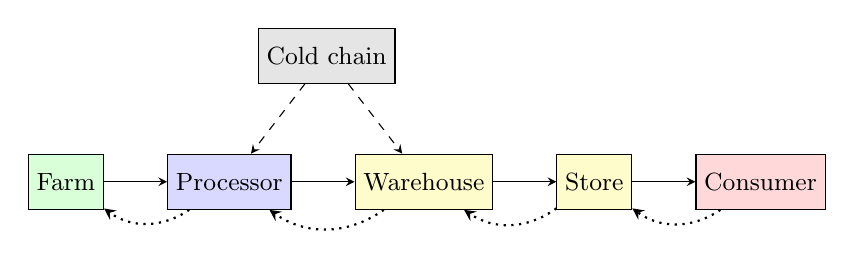
\begin{tikzpicture}[
    font=\small, >=stealth, node distance=0.8cm,
    box/.style={rectangle, draw, minimum height=0.7cm, inner sep=3pt}
]
    \node[box, fill=green!15] (farm) {Farm};
    \node[box, fill=blue!15, right=of farm] (proc) {Processor};
    \node[box, fill=yellow!20, right=of proc] (ware) {Warehouse};
    \node[box, fill=yellow!20, right=of ware] (store) {Store};
    \node[box, fill=red!15, right=of store] (cons) {Consumer};
    \node[box, fill=gray!20] (cold) at ($(proc)!0.5!(ware)+(0,1.6)$) {Cold chain};
    \draw[->] (farm) -- (proc);
    \draw[->] (proc) -- (ware);
    \draw[->] (ware) -- (store);
    \draw[->] (store) -- (cons);
    \draw[->, dashed] (cold) -- (proc);
    \draw[->, dashed] (cold) -- (ware);
    \draw[->, dotted, thick] (cons) to[bend left=35] (store);
    \draw[->, dotted, thick] (store) to[bend left=35] (ware);
    \draw[->, dotted, thick] (ware) to[bend left=35] (proc);
    \draw[->, dotted, thick] (proc) to[bend left=35] (farm);
\end{tikzpicture}
\caption{A food system network with parallel edges of different kinds: inventory (solid), service (dashed), and currency (dotted). A path computation with the kind filter $F=\{\text{inventory}\}$ uses only the solid edges.}
\label{fig:network}
\end{figure}

\subsection{Retained fraction of a component}

Every node and every edge is a component that acts on the quantity that reaches it. Below, $x$ denotes a component.

\begin{definition}[Transfer]\label{def:transfer}
The transfer of a component $x$ is a pair $(\hat w_x,c_x)\in[0,1]^2$. The component wastes the fraction $\hat w_x$ of its input and passes on the fraction $c_x$ of the remainder. The rest of the remainder, which is the fraction $(1-\hat w_x)(1-c_x)$ of the input, is the conversion shortfall. The retained fraction of $x$ is
\begin{equation}\label{eq:retained}
    r_x=(1-\hat w_x)\,c_x .
\end{equation}
\end{definition}

The effective waste rate $\hat w_x$ and the conversion $c_x$ follow from the stored parameters by the efficiency semantics of Section~\ref{sec:efficiency}. In the default mode, $c_x=1$, $\hat w_x=w_x$, and $r_x=1-w_x$.

\subsection{Efficiency semantics}\label{sec:efficiency}

Data sources report efficiency with different meanings. A mill reports the flour yield per tonne of wheat, which is a conversion ratio. A refrigerated transport operator may report the share of cargo that arrives in saleable condition, which is one minus a loss rate. EcoAnalyst makes the meaning explicit with an efficiency mode. The network has a default mode $\mu_0$, and a component can override it, so the mode of component $x$ is $m_x=\mu_x$ if $\mu_x$ is set and $m_x=\mu_0$ otherwise. With $w_x$ read as zero when it is unset, the three modes are
\begin{align}
    \text{ignore:}\quad & \hat w_x=w_x, && c_x=1, \label{eq:ignore}\\
    \text{conversion:}\quad & \hat w_x=w_x, && c_x=\eta_x, \label{eq:conversion}\\
    \text{retention:}\quad & \hat w_x=1-\eta_x, && c_x=1. \label{eq:retention}
\end{align}
In the ignore mode, which is the default, the efficiency is stored and not used. In the conversion mode the output is the input multiplied by $(1-w_x)\,\eta_x$. The shortfall $(1-w_x)(1-\eta_x)$ is reported separately and is not priced as waste. In the retention mode the efficiency is the fraction that gets through. If $w_x$ is also set, the two values must agree, and the library raises an error when $|1-\eta_x-w_x|>10^{-6}$. If $\eta_x$ is unset, every mode reduces to~\eqref{eq:ignore}.

A consistency check reports retention-mode components whose two values disagree. It also warns about conversion-mode components with $\eta_x=1-w_x$. That equality usually means that both fields describe the same loss, which the conversion mode would then count twice.

\subsection{Path loss}\label{sec:pathloss}

A path is a sequence of nodes $\pi=(v_0,\dots,v_k)$ in which every consecutive pair is joined by at least one edge whose kind is in $F$. Let $E_F(u,v)$ be the set of edges from $u$ to $v$ with kind in $F$. Between $v_{i-1}$ and $v_i$ the library uses the eligible edge that passes on the largest fraction,
\begin{equation}\label{eq:parallel}
    e_i=\arg\max_{e\in E_F(v_{i-1},v_i)} r_e .
\end{equation}
The path then has the component sequence
\[
    (x_1,\dots,x_{2k+1})=(v_0,e_1,v_1,\dots,e_k,v_k),
\]
which includes both end nodes. One unit of input enters $x_1$. Let $q_0=1$ and let $q_j=q_{j-1}\,r_{x_j}$ be the quantity that leaves component $x_j$.

\begin{definition}[Path fractions]\label{def:fractions}
The delivered fraction, the waste fraction, and the conversion fraction of $\pi$ are
\begin{align}
    D(\pi)&=q_{2k+1}=\prod_{j=1}^{2k+1} r_{x_j}, \label{eq:delivered}\\
    W(\pi)&=\sum_{j=1}^{2k+1} q_{j-1}\,\hat w_{x_j}, \label{eq:waste}\\
    C(\pi)&=\sum_{j=1}^{2k+1} q_{j-1}\,(1-\hat w_{x_j})(1-c_{x_j}). \label{eq:conv}
\end{align}
\end{definition}

\begin{lemma}[Balance]\label{lem:balance}
For every path, $D(\pi)+W(\pi)+C(\pi)=1$. If no component on $\pi$ converts, then $W(\pi)=1-\prod_{j}(1-\hat w_{x_j})$.
\end{lemma}
\begin{proof}
For each $j$,
\[
    q_{j-1}-q_j=q_{j-1}(1-r_{x_j})=q_{j-1}\hat w_{x_j}+q_{j-1}(1-\hat w_{x_j})(1-c_{x_j}).
\]
The sum over $j$ telescopes to $q_0-q_{2k+1}=1-D(\pi)=W(\pi)+C(\pi)$. If $c_{x_j}=1$ for all $j$, then $C(\pi)=0$ and $D(\pi)=\prod_j(1-\hat w_{x_j})$.
\end{proof}

Lemma~\ref{lem:balance} is the mass balance of a path: every unit of input is delivered, wasted, or converted. The functions \code{calculate\_path\_transfer} and \code{calculate\_path\_waste} return these fractions together with the contribution of each component. Each term in~\eqref{eq:waste} applies a loss rate to what reaches the component, not to the original input. A sum of the raw rates overstates the loss. For rates in $[0,1]$ the Weierstrass product inequality gives $\prod_j(1-w_j)\geq 1-\sum_j w_j$, so $\sum_j w_j\geq 1-\prod_j(1-w_j)$, with equality only when at most one rate is positive. The sum can also exceed one. For the four node rates 0.044, 0.050, 0.065, and 0.150 of Figure~\ref{fig:network_viz}, the sum is 0.309 and the compounded loss is $1-(0.956)(0.950)(0.935)(0.850)=0.278$.

\subsection{Minimum-loss routing}\label{sec:routing}

For a source $s$ and a target $t\neq s$, the function \code{find\_minimum\_waste\_path} returns the path that delivers the largest fraction. It first builds a simple directed graph $H$ on $N$. For each ordered pair $(u,v)$ with at least one eligible edge, let $r^*(u,v)=\max_{e\in E_F(u,v)} r_e$. If $r^*(u,v)>0$ and $r_u>0$, the graph $H$ contains the arc $(u,v)$ with weight
\begin{equation}\label{eq:weight}
    \omega(u,v)=-\ln r^*(u,v)-\ln r_u .
\end{equation}
An arc whose best edge or whose source node passes on nothing is left out.

\begin{proposition}[Minimum-loss routing]\label{prop:routing}
Assume $r_t>0$. Every $s$--$t$ path with $D(\pi)>0$ is a path in $H$, and every $s$--$t$ path $\pi=(v_0=s,\dots,v_k=t)$ in $H$ satisfies
\begin{equation}\label{eq:sumweight}
    \sum_{i=1}^{k}\omega(v_{i-1},v_i)=-\ln D(\pi)+\ln r_t .
\end{equation}
The weights are non-negative. A shortest $s$--$t$ path in $H$ therefore maximizes $D(\pi)$ over all $s$--$t$ paths, and Dijkstra's algorithm~\cite{dijkstra1959note} finds one. If no component converts, the same path minimizes the waste fraction $W(\pi)$.
\end{proposition}
\begin{proof}
A path with $D(\pi)>0$ has $r>0$ for every component, so each of its arcs is in $H$. By~\eqref{eq:parallel} the edge used between $v_{i-1}$ and $v_i$ has $r_{e_i}=r^*(v_{i-1},v_i)$. The logarithm turns the product~\eqref{eq:delivered} into a sum:
\[
    -\ln D(\pi)=-\sum_{i=0}^{k}\ln r_{v_i}-\sum_{i=1}^{k}\ln r_{e_i}
    =\sum_{i=1}^{k}\bigl(-\ln r_{e_i}-\ln r_{v_{i-1}}\bigr)-\ln r_t ,
\]
which is~\eqref{eq:sumweight}. The term $\ln r_t$ is the same for every path to $t$, and $-\ln$ is decreasing, so the path with the smallest weight sum has the largest $D(\pi)$. Every arc of $H$ has $r^*(u,v)\in(0,1]$ and $r_u\in(0,1]$, so $\omega(u,v)\geq 0$. Non-negative weights are the condition under which Dijkstra's algorithm returns a shortest path. If no component converts, Lemma~\ref{lem:balance} gives $W(\pi)=1-D(\pi)$.
\end{proof}

Building $H$ takes $O(|E|)$ time, and Dijkstra's algorithm with a binary heap takes $O((|N|+|A|)\log|N|)$ time, where $A$ is the arc set of $H$ and $|A|\leq|E|$. The function \code{find\_all\_paths} lists up to $K$ simple paths in order of increasing weight sum, which by~\eqref{eq:sumweight} is the order of decreasing delivered fraction. It uses Yen's algorithm~\cite{yen1971finding} as implemented in NetworkX.

\begin{remark}[What the routing does not model]\label{rem:routing}
When some component converts, the route maximizes the delivered fraction, and that route need not minimize waste. A path that wastes nothing but converts with $\eta=0.7$ delivers $0.7$ with $W=0$. A path with a single waste rate of $0.2$ delivers $0.8$ with $W=0.2$. The router chooses the second path.

The weights~\eqref{eq:weight} depend only on waste rates and efficiencies. Capacities $Q_v$, unit counts $n_v$, and maximum rates $M_e$ do not enter them. The computation follows a fraction of one unit along a single path, not a quantity of flow. The result is the best single path per unit of input, and that path may be unable to carry a given supply. Allocating a supply across several paths subject to capacities, with losses on the arcs, is a generalized network flow problem~\cite{ahuja1993network}. The library does not solve it.
\end{remark}

\section{Loss cost}\label{sec:cost}

Both cost estimates use a price $p(\ell)$ per unit for each node class $\ell$, with a default price for classes that have no price. An edge is priced by the class of its source node. Write $\ell_v$ for the class of node $v$.

The capacity-based estimate treats every component on its own and assumes that it runs at full capacity:
\begin{equation}\label{eq:lcap}
    L_{\mathrm{cap}}(\theta)=\sum_{v\in N} p(\ell_v)\,Q_v\,n_v\,\hat w_v+\sum_{e\in E} p(\ell_{\mathrm{src}(e)})\,M_e\,\hat w_e .
\end{equation}
This estimate does not follow material from one component to the next, so it is not a mass balance. It serves to rank components and to compare two versions of a network. The hotspot ranking uses the same component quantities.

The path estimate follows an input quantity $I$ along a path $\pi$. By default $I=Q_{v_0}n_{v_0}$. Component $x_j$ receives $I\,q_{j-1}$ and wastes $I\,q_{j-1}\hat w_{x_j}$, so
\begin{equation}\label{eq:lpath}
    L_{\mathrm{path}}(\pi)=I\sum_{j=1}^{2k+1} p_j\,q_{j-1}\,\hat w_{x_j},
\end{equation}
where $p_j$ is the price of the class of $x_j$, or of the source node of $x_j$ if $x_j$ is an edge. The delivered, wasted, and converted quantities are $I\,D(\pi)$, $I\,W(\pi)$, and $I\,C(\pi)$. The conversion shortfall is reported and is not priced. The two estimates answer different questions and in general give different values: $L_{\mathrm{cap}}$ charges every component at capacity, including components that a given path does not use, while $L_{\mathrm{path}}$ charges only the components on $\pi$ and only for what reaches them.

The library also computes a total cost of ownership over $Y$ years at a discount rate $d$,
\begin{equation}\label{eq:tco}
    \mathrm{TCO}=K+J+\sum_{y=1}^{Y}\frac{O}{(1+d)^{y}}-\frac{S}{(1+d)^{Y}},
\end{equation}
where $K$, $J$, $O$, and $S$ are the capital, installation, annual operating, and salvage values summed over the nodes.

\section{The 1.x modules and associational analysis}\label{sec:legacy}

The modules of version 1.x remain in the subpackage \code{ecoanalyst.legacy} so that existing scripts keep working. This section describes their network model and their regression module.

\subsection{Typed nodes and loss functions}

The class \code{AdvancedWasteNetwork} represents actors with typed classes (initial producer, food processor, food handler, end consumer, and solution provider) joined by inventory, service, and currency edges. It rejects inventory edges into an initial producer and inventory edges out of an end consumer. Each node and edge has a loss function that is evaluated on the current conditions:
\begin{align}
    \text{static:}\quad & w_s=\alpha, \label{eq:static}\\
    \text{time-based:}\quad & w_t(t)=\beta_0+\beta_1 t, \label{eq:timebased}\\
    \text{multivariable:}\quad & w_m(\mathbf{x})=f(\mathbf{x}), \label{eq:multivar}\\
    \text{regression-based:}\quad & w_r(\mathbf{x})=\min\bigl(1,\max(0,\hat\alpha+\mathbf{x}^{\top}\hat{\boldsymbol\beta})\bigr), \label{eq:regloss}
\end{align}
where $t$ is a time in the units of $\beta_1$, $f$ is a user function, and $(\hat\alpha,\hat{\boldsymbol\beta})$ are posterior mean coefficients from Section~\ref{sec:regression}. The path computation evaluates the functions at $t=24$ unless the caller gives another time, clamps each loss to $[0,1]$, uses the inventory edge with the lowest loss between consecutive nodes, and compounds the losses as in Lemma~\ref{lem:balance} without conversion. Its routing uses the weights $-\ln(1-w_e)$ on edge losses only. Its arguments for a custom cost function and for capacity constraints are accepted and not used.

Solution providers and service edges store an effect multiplier $\alpha_s\in(0,1]$, and processors store transformation rules for output composition. No loss calculation applies either of them. In version 3.0 the effect of a service on a loss rate is expressed in the causal graph of Section~\ref{sec:causal}, where a variable for the service is a parent of the variable bound to the loss rate.

\begin{figure}[htbp]
\centering
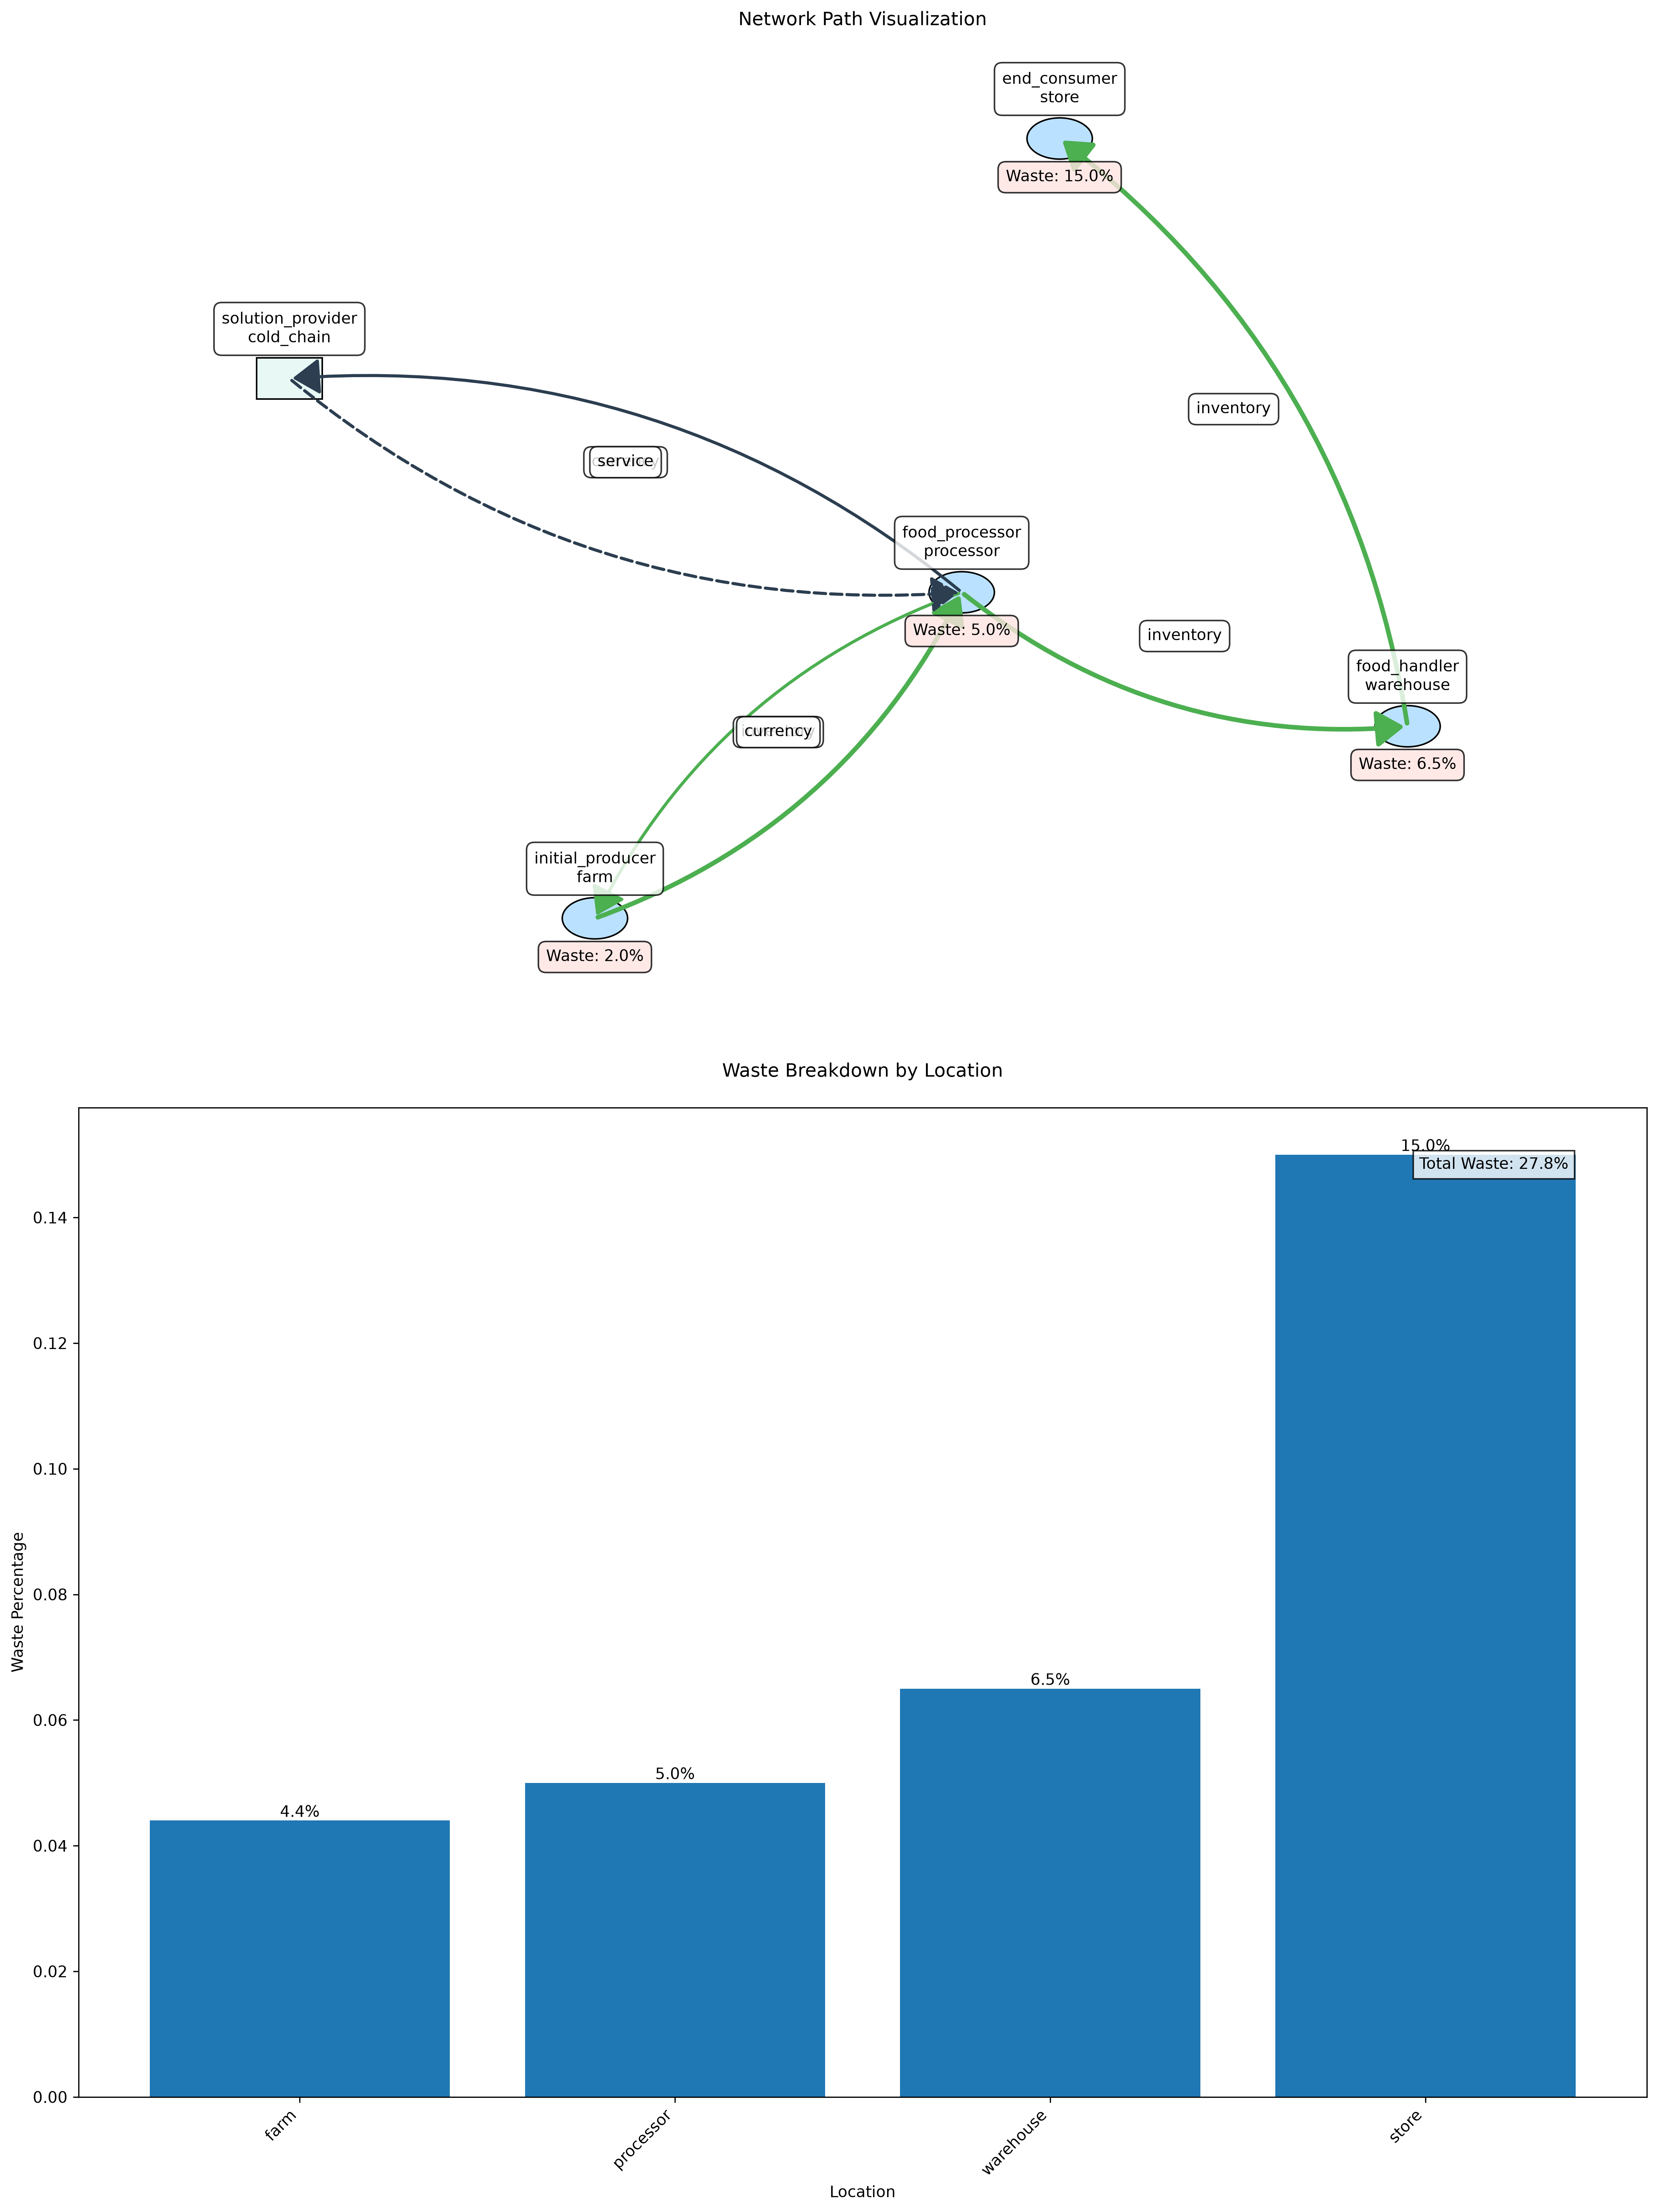
\includegraphics[width=0.5\textwidth]{../data/network_visualization.png}
\caption{Drawing produced by the 1.x drawing helpers (\code{examples/network\_visualization.py}) for the path farm, processor, warehouse, store. The farm uses the time-based loss~\eqref{eq:timebased} with 2\% plus 0.1\% per hour, evaluated at 24 hours. The processor and the store use static losses, and the warehouse uses a function of temperature and humidity. The node labels show each component's base rate, so the farm reads 2.0\% in the graph and 4.4\% in the bar chart. The total printed in the chart, 27.8\%, compounds the four evaluated rates as in Lemma~\ref{lem:balance}.}
\label{fig:network_viz}
\end{figure}

\subsection{Bayesian regression of loss on its drivers}\label{sec:regression}

The class \code{WasteCausalNetwork} keeps its 1.x name for compatibility. For a loss column $y$ and driver columns $\mathbf{x}$ it fits the linear model
\begin{gather*}
    y_i \sim \mathcal{N}(\alpha+\mathbf{x}_i^{\top}\boldsymbol\beta,\ \sigma^2),\\
    \alpha \sim \mathcal{N}(0,10^2),\qquad
    \beta_j \sim \mathcal{N}(0,2^2),\qquad
    \sigma \sim \text{Half-Normal}(1),
\end{gather*}
and, for a binary outcome, the logistic model $y_i\sim\text{Bernoulli}\bigl(\expit(\alpha+\mathbf{x}_i^{\top}\boldsymbol\beta)\bigr)$ with the same priors on $\alpha$ and $\boldsymbol\beta$. The posterior is sampled by Markov chain Monte Carlo in PyMC~\cite{pymc}. The method \code{fit\_regression} standardizes each driver to zero mean and unit variance, so its coefficients are per standard deviation of the driver. The method \code{fit} keeps the drivers on their original scale, so that the regression-based loss function~\eqref{eq:regloss} can apply the coefficients to raw values.

The two methods report different intervals. The method \code{fit\_regression} reports, for each record, the central 95\% interval of the posterior draws of $\alpha+\mathbf{x}_i^{\top}\boldsymbol\beta$. This interval describes uncertainty about the mean loss and excludes the noise $\sigma$. The method \code{fit} reports $\hat y_i\pm 1.96\,s$, where $\hat y_i$ uses the posterior mean coefficients and $s$ is the standard deviation of the residuals.

\subsection{Interpretation}\label{sec:assoc}

The posterior of $\beta_j$ summarizes how the expected loss differs between records that differ in $x_j$ and agree on the other included drivers. This is a property of the joint distribution that generated the data. It equals the effect of changing $x_j$ by intervention only if two further conditions hold: the other included drivers block every back-door path from $x_j$ to the loss (Section~\ref{sec:identification}), and the linear form is correct. The module checks neither condition, so its output is associational.

Two methods keep 1.x names and do not estimate causal quantities. The method \code{get\_causal\_effect} returns the product of user-supplied edge weights along the shortest path between two variables, together with the bootstrap standard deviation of a Pearson correlation. The method \code{discover\_causal\_structure} joins two columns when their marginal Pearson correlation is significant at a chosen level, and it orients each edge from the column name that sorts later to the one that sorts earlier.

\subsection{Example with simulated drivers}\label{sec:toy}

The script \code{examples/toy\_ecosystem.py} simulates 1000 records with three independent drivers, temperature $T\sim\mathcal{N}(20,5^2)$, humidity $H\sim\mathcal{N}(50,10^2)$, and storage time $S\sim\mathcal{N}(24,6^2)$. An unobserved damage variable is $U=0.3T+0.2H+0.4S+\varepsilon_1$, and the recorded waste is $Y=0.8U+\varepsilon_2$, with $\varepsilon_1,\varepsilon_2\sim\mathcal{N}(0,1)$. The implied slopes of $\mathbb{E}[Y\mid T,H,S]$ are $0.24$, $0.16$, and $0.32$. The regression of $Y$ on $(T,H,S)$ with \code{fit} gives posterior means $0.231$, $0.153$, and $0.329$, with posterior standard deviations $0.009$, $0.004$, and $0.007$, and $R^2=0.812$. Figure~\ref{fig:causal_analysis} shows the variable graph that the script builds, with the simulation coefficients as edge weights.

The agreement between the estimates and the simulated weights follows from the design of the simulation. The drivers are drawn independently, and no variable affects both a driver and the waste, so the conditional expectation coincides with the interventional one. In records collected during operation, a common cause such as the season can affect both storage time and temperature. The regression coefficients then do not have this interpretation unless the adjustment conditions of Section~\ref{sec:identification} hold.

\begin{figure}[htbp]
\centering
\includegraphics[width=0.7\textwidth]{../data/causal_network.png}
\caption{Variable graph drawn by the 1.x regression module for the simulated data of Section~\ref{sec:toy}. The edge labels are the weights passed to \code{add\_edge}, which are the coefficients used to simulate the data. The module stores these weights and does not estimate them. The graph records the association structure assumed between storage conditions and waste. The title inside the image is the name of the 1.x class.}
\label{fig:causal_analysis}
\end{figure}

\section{A causal graph in parallel to the flow graph}\label{sec:causal}

The flow network answers questions of the form ``given these loss rates, how much arrives''. The module \code{ecoanalyst.causal} adds a second graph that answers ``why do the loss rates take these values, and how do they change under an intervention''. The two graphs stay separate. They are connected only through bindings from causal variables to parameters of the flow network.

\subsection{Two graphs and a binding map}\label{sec:binding}

\begin{definition}[Causal graph]\label{def:causal}
A causal graph is a directed acyclic graph (DAG) $G_c=(V,A)$ over a finite set of variables $V$. Each variable $X\in V$ has a kind $k_X\in\{\text{continuous},\text{rate},\text{positive},\text{binary}\}$, a parent set $\Pa(X)=\{P:(P,X)\in A\}$, and a flag that marks it as observed or unobserved.
\end{definition}

Variables are added parents first. The insertion order is therefore a topological order, and the graph is acyclic by construction.

\begin{definition}[Binding map]\label{def:bindingmap}
A binding map is an injective map $\phi$ from a subset $V_B\subseteq V$ to coordinates of $\theta$. The admissible coordinates are the node waste rate, efficiency, and degradation rate, which require a rate variable, the node capacity, which requires a positive variable, the edge waste rate and efficiency, which require a rate variable, and the edge maximum rate, which requires a positive variable. For values $V=\mathbf{v}$, the bound parameter vector $\theta(\mathbf{v})$ equals $\theta$ except that coordinate $\phi(X)$ takes the value $v_X$ for every $X\in V_B$. The bound network is $G_p[\theta(\mathbf{v})]$.
\end{definition}

The library refuses to simulate when a binding names a node or edge that is not in the network, or when two variables drive the same coordinate. A bound coordinate affects an outcome only if the outcome reads it. Capacity and maximum rate enter only the capacity-based cost~\eqref{eq:lcap}. An efficiency matters only in the conversion and retention modes. No calculation in version 3.0 reads the degradation rate. Figure~\ref{fig:coupled} in Section~\ref{sec:example} shows a causal graph with two bindings.

\subsection{Structural equations}\label{sec:equations}

Each variable $X$ has a linear predictor on its link scale,
\begin{equation}\label{eq:linpred}
    \eta_X=\beta_{X,0}+\sum_{P\in\Pa(X)}\beta_{X,P}\,P ,
\end{equation}
in which the parents enter on their natural scale. With $\varepsilon_X\sim\mathcal{N}(0,1)$, $U_X\sim\mathrm{Uniform}(0,1)$, and a noise scale $s_X\geq 0$, the structural equation of $X$ depends on its kind as shown in Table~\ref{tab:kinds}. A rate variable is therefore logit-normal given its parents, and a positive variable is log-normal given its parents. The coefficients $\boldsymbol\beta_X=(\beta_{X,0},(\beta_{X,P})_{P\in\Pa(X)})$ and the scale $s_X$ are either stated by the user or drawn from the posterior of Section~\ref{sec:update}. A stated intercept is given on the link scale. For example, a rate variable with no parents and the intercept $\logit(0.05)$ has a median of 5\%.

\begin{table}[htbp]
\centering
\small
\begin{tabular}{llll}
\toprule
Kind & Link $h$ & Values & Structural equation \\
\midrule
continuous & identity & $\mathbb{R}$ & $X=\eta_X+s_X\varepsilon_X$ \\
rate & logit & $(0,1)$ & $X=\expit(\eta_X+s_X\varepsilon_X)$ \\
positive & log & $(0,\infty)$ & $X=\exp(\eta_X+s_X\varepsilon_X)$ \\
binary & logit & $\{0,1\}$ & $X=\mathbf{1}\{U_X<\expit(\eta_X)\}$ \\
\bottomrule
\end{tabular}
\caption{Variable kinds, link functions, and structural equations. Here $\expit(z)=1/(1+e^{-z})$, and the exogenous terms $\varepsilon_X$ and $U_X$ are independent across variables.}
\label{tab:kinds}
\end{table}

\subsection{Outcomes}\label{sec:outcomes}

An outcome is computed for each joint sample. A flow outcome is a function $g$ of the parameter vector, evaluated on the bound network: $Y=g\bigl(G_p[\theta(V)]\bigr)$. The library provides the following flow outcomes:
\begin{itemize}
    \item the waste fraction $W(\pi)$ and the delivered fraction $D(\pi)$ of a fixed path $\pi$;
    \item the delivered fraction $D(\pi^*(\theta))$ of the best route, where $\pi^*(\theta)$ is the route of Proposition~\ref{prop:routing}, recomputed for every parameter vector (the value is $0$ when no route exists);
    \item the path loss cost $L_{\mathrm{path}}(\pi)$ and the capacity-based cost $L_{\mathrm{cap}}$.
\end{itemize}
An outcome can also be the value of a causal variable. The flow outcome is evaluated separately for each sample, so $g$ can be any function of $\theta$. The best-route outcome, for example, is continuous but not differentiable at parameter values where the best route changes.

\subsection{Sampling and interventions}\label{sec:sampling}

Ancestral sampling draws $n$ joint samples. For each sample, the sampler visits the variables in topological order and computes each variable from the values already drawn for its parents and from fresh exogenous terms. The Monte Carlo estimate of the expected outcome is
\begin{equation}\label{eq:mc}
    \widehat{\mathbb{E}}[g]=\frac{1}{n}\sum_{i=1}^{n} g\bigl(G_p[\theta(\mathbf{v}^{(i)})]\bigr).
\end{equation}
The library sets the bound parameters for each sample, evaluates the outcome, and restores the original values afterwards.

An intervention $do(X=x)$ replaces the structural equation of $X$ with the constant $x$. In the graph this deletes every arrow into $X$, which is the graph surgery of Pearl~\cite{pearl2009causality}. The result is the interventional distribution $P(V\mid do(X=x))$. Several variables can be set at once. The value is checked against the kind of the variable: a rate must lie in $[0,1]$, a positive value must be greater than zero, and a binary value must be $0$ or $1$. An intervention on a bound variable fixes the corresponding network parameter. An intervention on an upstream variable changes the bound parameters through every directed path from that variable.

\subsection{Effect estimation with shared exogenous noise}\label{sec:effect}

For two sets of interventions $a$ and $b$, the effect on the outcome $g$ is
\begin{equation}\label{eq:estimand}
    \tau(a,b)=\mathbb{E}\bigl[g(G_p[\theta(V)])\mid do(a)\bigr]-\mathbb{E}\bigl[g(G_p[\theta(V)])\mid do(b)\bigr].
\end{equation}
The set $b$ may be empty, and then the second term is the expectation under the unmodified model.

The function \code{compare} estimates $\tau(a,b)$ with common random numbers (Algorithm~\ref{alg:compare}). For every variable, and in the same order, the sampler draws the same random numbers whether or not the variable is set by an intervention. With the same seed, sample $i$ under $a$ and sample $i$ under $b$ therefore share their exogenous terms and their parameter draws, and they differ only through the interventions. The estimate is
\begin{equation}\label{eq:tauhat}
    \hat\tau=\frac{1}{n}\sum_{i=1}^{n}\Delta_i,\qquad \Delta_i=g_a^{(i)}-g_b^{(i)},
\end{equation}
with variance $\operatorname{Var}(\hat\tau)=\bigl(\operatorname{Var}(g_a)+\operatorname{Var}(g_b)-2\operatorname{Cov}(g_a,g_b)\bigr)/n$. Independent draws for the two regimes would make the covariance zero. When $g_a$ and $g_b$ respond in the same direction to the shared terms, the covariance is non-negative, and the variance of $\hat\tau$ is no larger than with independent draws. The library reports $\hat\tau$, the 5th, 50th, and 95th percentiles of $\Delta_i$, and the share of samples with $\Delta_i>0$. The percentiles describe how the effect varies across samples, that is, across exogenous conditions and parameter draws. They are not a credible interval for $\tau$.

\begin{algorithm}[htbp]
\caption{Estimate of $\tau(a,b)$ with shared exogenous noise}
\label{alg:compare}
\begin{algorithmic}[1]
\REQUIRE causal graph $G_c$ with equations, flow network $G_p$ with parameters $\theta$, binding map $\phi$, outcome $g$, intervention sets $a$ and $b$, sample size $n$, seed
\FOR{each regime $\rho\in\{a,b\}$}
    \STATE start the random number generator from the seed
    \FOR{each variable $X$ in topological order}
        \STATE draw, for all $n$ samples, the coefficient normals, $\varepsilon_X$, $U_X$, and (for a fitted normal-inverse-gamma posterior) a gamma variate for $s_X^2$
        \IF{$\rho$ sets $X$ to $x$}
            \STATE $X^{(i)}\gets x$ for all $i$
        \ELSE
            \STATE compute $X^{(i)}$ from its equation, the parent values $\Pa(X)^{(i)}$, and the draws
        \ENDIF
    \ENDFOR
    \STATE $g_\rho^{(i)}\gets g\bigl(G_p[\theta(\mathbf{v}^{(i)})]\bigr)$ for $i=1,\dots,n$
\ENDFOR
\STATE $\Delta_i\gets g_a^{(i)}-g_b^{(i)}$
\RETURN the mean of $\Delta$, its 5th, 50th, and 95th percentiles, and the share of $\Delta_i>0$
\end{algorithmic}
\end{algorithm}

When the posterior of an equation is used, each sample draws its own coefficients (Section~\ref{sec:update}). The average~\eqref{eq:tauhat} then estimates the posterior mean of $\tau$, and the spread of $\Delta_i$ combines parameter uncertainty with exogenous variation. With parameter uncertainty switched off, every sample uses the posterior mean.

\subsection{Bayesian update}\label{sec:update}

The function \code{fit} updates the equation of a variable $X$ when the data contain a column for $X$ and for each of its parents. It skips rows with a missing or non-finite value in any of these columns, and it leaves the other variables with their stated equations. Let $Z$ be the $n\times p$ design matrix with a column of ones and one column per parent, and let $\mathbf{y}=h(\mathbf{x})$ be the observed values of $X$ on the link scale. Rate values are clipped to $[10^{-9},1-10^{-9}]$ before the logit.

\paragraph{Continuous, rate, and positive variables.}
The prior is normal-inverse-gamma,
\begin{equation}\label{eq:nigprior}
    \boldsymbol\beta\mid s^2\sim\mathcal{N}\bigl(\mathbf{m}_0,\ s^2\Lambda_0^{-1}\bigr),\qquad s^2\sim\text{Inv-Gamma}\bigl(a_0,b_0\bigr),
\end{equation}
with
\begin{equation}\label{eq:autoscale}
    \Lambda_0=\lambda^{-2}\operatorname{diag}\bigl(1,\sigma_1^2,\dots,\sigma_{p-1}^2\bigr),\qquad a_0=2,\qquad b_0=s_0^2.
\end{equation}
Here $\mathbf{m}_0$ holds the stated intercept and coefficients, $\lambda$ is a prior scale with default value 10, $\sigma_j$ is the sample standard deviation of the $j$th parent over the rows used (1 for a constant column), and $s_0$ is the sample standard deviation of $\mathbf{y}$. The prior standard deviation of the coefficient of parent $j$ is therefore $\lambda s/\sigma_j$, that is, $\lambda$ noise scales per standard deviation of the parent, and $\mathbb{E}[s^2]=b_0/(a_0-1)=s_0^2$. Both scales come from the data, so the prior carries the same weight whatever the units: a variable or a parent measured in other units gives the same fit expressed in those units. A prior with fixed scales does not have this property. For monthly changes of a logarithm, for example, the residual scale is of order $10^{-3}$, and a prior noise scale of 1 then dominates $b_n$ and inflates the noise scale by an order of magnitude. The option \code{autoscale=False} uses $\Lambda_0=\lambda^{-2}I_p$ and the stated noise scale as $s_0$. The posterior is normal-inverse-gamma with~\cite{gelman2013bda}
\begin{align}
    \Lambda_n&=\Lambda_0+Z^{\top}Z, &
    \mathbf{m}_n&=\Lambda_n^{-1}\bigl(\Lambda_0\mathbf{m}_0+Z^{\top}\mathbf{y}\bigr), \label{eq:nigpost1}\\
    a_n&=a_0+\tfrac{n}{2}, &
    b_n&=b_0+\tfrac12\bigl(\mathbf{y}^{\top}\mathbf{y}+\mathbf{m}_0^{\top}\Lambda_0\mathbf{m}_0-\mathbf{m}_n^{\top}\Lambda_n\mathbf{m}_n\bigr). \label{eq:nigpost2}
\end{align}
This posterior is exact. To draw the parameters for one sample, the library computes
\begin{align*}
    s^2&=b_n/G, && G\sim\text{Gamma}(a_n,1),\\
    \boldsymbol\beta&=\mathbf{m}_n+s\,L\mathbf{z}, && LL^{\top}=\Lambda_n^{-1},\quad \mathbf{z}\sim\mathcal{N}(0,I_p),
\end{align*}
so that $s^2\sim\text{Inv-Gamma}(a_n,b_n)$. Without parameter uncertainty it uses $\mathbf{m}_n$ and the noise scale $\sqrt{b_n/(a_n-1)}$.

\paragraph{Binary variables.}
The prior is $\boldsymbol\beta\sim\mathcal{N}(\mathbf{m}_0,\Lambda_0^{-1})$ with $\Lambda_0$ from~\eqref{eq:autoscale}, so the prior standard deviation of the coefficient of parent $j$ is $\lambda/\sigma_j$ on the logit scale. Newton's method finds the posterior mode $\hat{\boldsymbol\beta}$ with the gradient and Hessian of the negative log posterior $\ell$,
\begin{align}
    \nabla\ell(\boldsymbol\beta)&=Z^{\top}(\mathbf{p}-\mathbf{y})+\Lambda_0(\boldsymbol\beta-\mathbf{m}_0), \nonumber\\
    \nabla^2\ell(\boldsymbol\beta)&=Z^{\top}\operatorname{diag}\bigl(\mathbf{p}\odot(1-\mathbf{p})\bigr)Z+\Lambda_0, \label{eq:newton}
\end{align}
where $\mathbf{p}=\expit(Z\boldsymbol\beta)$. It stops after 100 iterations or when the largest step is below $10^{-10}$. The Laplace approximation to the posterior is $\boldsymbol\beta\mid\text{data}\approx\mathcal{N}\bigl(\hat{\boldsymbol\beta},[\nabla^2\ell(\hat{\boldsymbol\beta})]^{-1}\bigr)$~\cite{gelman2013bda}.

When all variables are observed, the exogenous terms are independent, and the priors of different equations are independent, the likelihood of the data factorizes into one factor per variable, $\prod_{X\in V}p\bigl(x\mid\Pa(X),\boldsymbol\beta_X,s_X\bigr)$. Fitting each equation separately then gives the joint posterior. The library does not integrate over unobserved variables. An unobserved variable has no column in the data, so neither its own equation nor the equations of its children can be fitted, and those equations keep their stated values.

\subsection{Identification}\label{sec:identification}

An effect computed by Algorithm~\ref{alg:compare} is the effect implied by the model. It is identified from observational data only under assumptions about the graph. Two results apply.

\paragraph{Truncated factorization.}
Suppose that every variable is observed and that assumptions (A1), (A2), and (A5) of Section~\ref{sec:assumptions} hold. For an intervention $do(X=x)$ and values $\mathbf{v}$ with $v_X=x$, the interventional distribution is~\cite{pearl2009causality}
\begin{equation}\label{eq:truncated}
    P\bigl(\mathbf{v}\mid do(X=x)\bigr)=\prod_{V_j\in V\setminus\{X\}}P\bigl(v_j\mid \mathrm{pa}_j\bigr),
\end{equation}
and it is zero for values with $v_X\neq x$. Here $\mathrm{pa}_j$ denotes the values of $\Pa(V_j)$ in $\mathbf{v}$. Each factor is a conditional distribution of observed variables, which \code{fit} estimates from observational data. Sampling with the equation of $X$ replaced draws from this product. Under (A3) and (A4) for the support and form of each factor, the effect~\eqref{eq:estimand} is therefore identified.

\paragraph{Back-door criterion.}
When some variables are unobserved, the simulation relies on stated equations for their children. The library can still report whether an effect is estimable from observational data by adjustment.

\begin{definition}[Back-door criterion~\cite{pearl1995causal}]\label{def:backdoor}
A set $\mathbf{Z}\subseteq V\setminus\{X,Y\}$ satisfies the back-door criterion relative to $(X,Y)$ if no element of $\mathbf{Z}$ is a descendant of $X$ and $\mathbf{Z}$ blocks every path between $X$ and $Y$ that contains an arrow into $X$.
\end{definition}

\begin{theorem}[Back-door adjustment~\cite{pearl1995causal,pearl2009causality}]\label{thm:backdoor}
If $\mathbf{Z}$ satisfies the back-door criterion relative to $(X,Y)$, then
$P\bigl(y\mid do(X=x)\bigr)=\sum_{\mathbf{z}}P(y\mid x,\mathbf{z})\,P(\mathbf{z})$.
\end{theorem}

The function \code{is\_valid\_adjustment}$(X,Y,\mathbf{Z})$ returns true if and only if every element of $\mathbf{Z}$ is observed, $\mathbf{Z}\cap(\{X,Y\}\cup\De(X))=\emptyset$, and $\mathbf{Z}$ d-separates $X$ and $Y$ in the graph $G_{\underline{X}}$ obtained from $G_c$ by deleting the arrows out of $X$. The last condition is equivalent to blocking every back-door path. The function \code{adjustment\_set}$(X,Y)$ returns a minimal set of observed non-descendants of $X$ with this property, computed with the minimal d-separator routine of NetworkX. It returns the empty set when no adjustment is needed, and it returns \code{None} when no set of observed variables satisfies the criterion. The back-door criterion is sufficient and not necessary. When it fails, the effect can still be identifiable by other means, such as the front-door criterion, which the library does not check. The result tells a user which observed variables an estimate from data must condition on. That estimate can come from an outside regression or from DoWhy~\cite{sharma2020dowhy}, which reads the graph that \code{to\_gml} exports in GML.

\subsection{Assumptions}\label{sec:assumptions}

The effects that the causal layer reports are causal effects only under the following assumptions. The library does not test them.
\begin{enumerate}[label=(A\arabic*), leftmargin=*]
    \item \emph{The DAG is correct.} Every direct effect among the modeled variables is an arrow in $G_c$, and every missing arrow is a claim of no direct effect.
    \item \emph{No unmodeled common causes.} Every common cause of two modeled variables is itself in $V$. A common cause that is not measured must be included and marked unobserved.
    \item \emph{Positivity.} The intervention values, and each stratum of an adjustment set, have support in the data. Outside the observed range the simulation extrapolates the linear predictor on the link scale.
    \item \emph{Functional form.} Each equation is linear on its link scale in the natural-scale values of the parents, without interaction terms, with Gaussian noise on the link scale for continuous, rate, and positive variables and a logistic model for binary variables.
    \item \emph{Independent exogenous noise.} The terms $\varepsilon_X$ and $U_X$ are independent across variables, and the rows used by \code{fit} are independent draws.
\end{enumerate}
The structure of the flow network and its unbound parameters are held fixed. An intervention acts on the flow network only through the bound parameters.

\section{Worked example: a produce cold chain}\label{sec:example}

The script \code{examples/causal\_cold\_chain.py} builds the network and the causal graph of Figure~\ref{fig:coupled}. The numbers in this section come from that script, run with version 3.0.0 of the library, and from further calls on the network and model objects that it builds.

\begin{figure}[htbp]
\centering
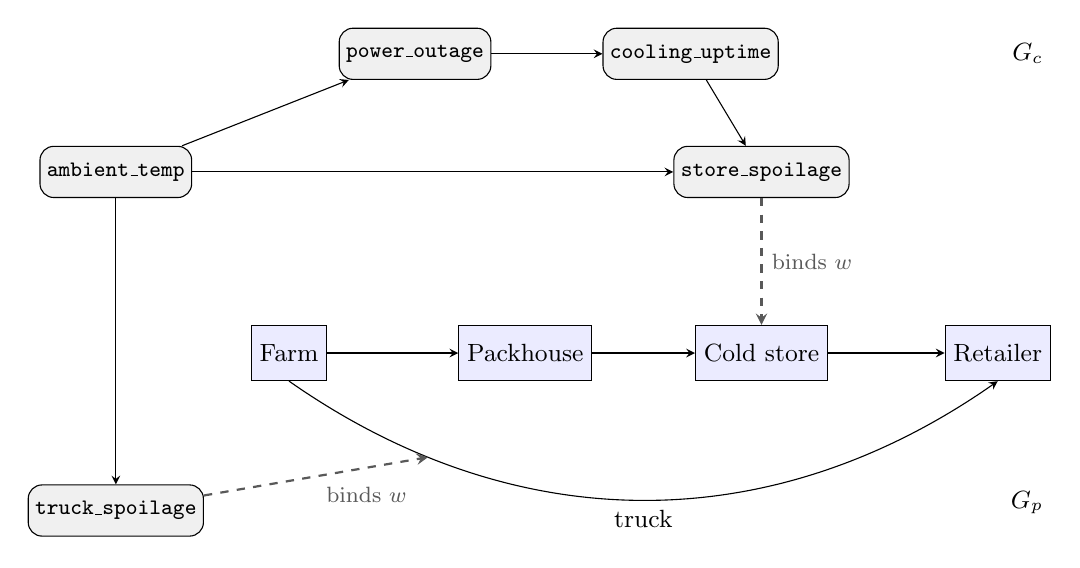
\begin{tikzpicture}[
    font=\small, >=stealth,
    cvar/.style={rectangle, rounded corners=5pt, draw, fill=gray!12, minimum height=0.65cm, inner sep=2.5pt, font=\footnotesize\ttfamily},
    fnode/.style={rectangle, draw, fill=blue!8, minimum height=0.7cm, inner sep=3pt},
    bind/.style={->, dashed, thick, black!65}
]
    % flow network
    \node[fnode] (farm) at (0.9,0) {Farm};
    \node[fnode] (pack) at (3.9,0) {Packhouse};
    \node[fnode] (store) at (6.9,0) {Cold store};
    \node[fnode] (shop) at (9.9,0) {Retailer};
    \draw[->] (farm) -- (pack);
    \draw[->] (pack) -- (store);
    \draw[->] (store) -- (shop);
    \draw[->] (farm.south) to[out=-35, in=-145] node[pos=0.5, below] {truck} coordinate[pos=0.2] (truckpt) (shop.south);
    % causal graph
    \node[cvar] (temp) at (-1.3,2.3) {ambient\_temp};
    \node[cvar] (outage) at (2.5,3.8) {power\_outage};
    \node[cvar] (uptime) at (6.0,3.8) {cooling\_uptime};
    \node[cvar] (ssp) at (6.9,2.3) {store\_spoilage};
    \node[cvar] (tsp) at (-1.3,-2.0) {truck\_spoilage};
    \draw[->] (temp) -- (outage);
    \draw[->] (outage) -- (uptime);
    \draw[->] (uptime) -- (ssp);
    \draw[->] (temp) -- (ssp);
    \draw[->] (temp) -- (tsp);
    \draw[bind] (ssp) -- node[right, font=\footnotesize] {binds $w$} (store);
    \draw[bind] (tsp) -- node[below right, font=\footnotesize] {binds $w$} (truckpt);
    \node[anchor=east] at (10.6,3.8) {$G_c$};
    \node[anchor=east] at (10.6,-1.9) {$G_p$};
\end{tikzpicture}
\caption{Causal graph $G_c$ (rounded boxes) in parallel to the flow network $G_p$ (square boxes) for the cold-chain example. Solid arrows between rounded boxes are causal arrows; solid arrows between square boxes are inventory edges. The dashed arrows are bindings: \code{store\_spoilage} drives the waste rate of the cold store, and \code{truck\_spoilage} drives the waste rate of the direct truck edge.}
\label{fig:coupled}
\end{figure}

\paragraph{Flow network.}
A farm ($w=0.02$) ships produce to a retailer ($w=0.04$) on one of two routes. The first route passes a packhouse ($w=0.01$, $\eta=0.90$) and a cold store ($w=0.03$), with $w=0.01$ on each of its three edges. The second route is a direct unrefrigerated truck with $w=0.20$. The network default mode is conversion, so the packhouse trims 10\% of what it keeps. At these stated values the cold-chain route has
\begin{gather*}
    D=0.98\cdot0.99\cdot(0.99\cdot0.90)\cdot0.99\cdot0.97\cdot0.99\cdot0.96=0.789,\\
    W=0.115,\qquad C=0.096,
\end{gather*}
and the truck route has $D=0.98\cdot0.80\cdot0.96=0.753$ and $W=0.247$. Proposition~\ref{prop:routing} therefore selects the cold-chain route.

\paragraph{Causal graph.}
The graph has five variables: \code{ambient\_temp} (continuous, in $^\circ$C), \code{power\_outage} (binary), \code{cooling\_uptime} (rate), \code{store\_spoilage} (rate, bound to the waste rate of the cold store), and \code{truck\_spoilage} (rate, bound to the waste rate of the truck edge). The stated equations serve as the prior. Their intercepts are $24$ for temperature, $\logit(0.95)$ for uptime, $\logit(0.03)$ for store spoilage, and $\logit(0.20)$ for truck spoilage, and their coefficients are zero.

\paragraph{Data and fit.}
The script generates 365 synthetic daily records from
\begin{align*}
    T&\sim\mathcal{N}(24,4^2),\\
    O&\sim\text{Bernoulli}\bigl(\expit(-9+0.25\,T)\bigr),\\
    U_c&=\expit(3.5-3\,O+0.3\,\varepsilon_1),\\
    S_s&=\expit(-3+0.08\,T-4\,U_c+0.2\,\varepsilon_2),\\
    S_t&=\expit(-3.8+0.10\,T+0.2\,\varepsilon_3),
\end{align*}
where $T$, $O$, $U_c$, $S_s$, and $S_t$ are temperature, outage, uptime, store spoilage, and truck spoilage, and $\varepsilon_1,\varepsilon_2,\varepsilon_3\sim\mathcal{N}(0,1)$. The records contain 20 outage days and 7 days at or above $32\,^\circ$C. All five equations are fitted. Table~\ref{tab:fit} compares the posterior means with the generating values.

\begin{table}[htbp]
\centering
\small
\begin{tabular}{llrr}
\toprule
Equation & Term & Generating value & Posterior mean \\
\midrule
\code{ambient\_temp} & intercept & 24 & 23.964 \\
 & noise scale & 4 & 3.761 \\
\code{power\_outage} & intercept & $-9.0$ & $-8.399$ \\
 & \code{ambient\_temp} & 0.25 & 0.219 \\
\code{cooling\_uptime} & intercept & 3.5 & 3.502 \\
 & \code{power\_outage} & $-3.0$ & $-3.053$ \\
 & noise scale & 0.3 & 0.302 \\
\code{store\_spoilage} & intercept & $-3.0$ & $-2.804$ \\
 & \code{ambient\_temp} & 0.08 & 0.073 \\
 & \code{cooling\_uptime} & $-4.0$ & $-4.037$ \\
 & noise scale & 0.2 & 0.209 \\
\code{truck\_spoilage} & intercept & $-3.8$ & $-3.891$ \\
 & \code{ambient\_temp} & 0.10 & 0.103 \\
 & noise scale & 0.2 & 0.206 \\
\bottomrule
\end{tabular}
\caption{Fitted equations of the cold-chain example on the link scale (365 records). The noise scale column shows $\sqrt{b_n/(a_n-1)}$. The binary equation for \code{power\_outage} uses the Laplace approximation and has no noise scale.}
\label{tab:fit}
\end{table}

\paragraph{Identification.}
For the effect of \code{cooling\_uptime} on \code{store\_spoilage}, the only back-door path is
\[
    \text{\code{cooling\_uptime}}\leftarrow\text{\code{power\_outage}}\leftarrow\text{\code{ambient\_temp}}\rightarrow\text{\code{store\_spoilage}}.
\]
The function \code{adjustment\_set} returns the set \{\code{power\_outage}\}. The set \{\code{ambient\_temp}\} also satisfies the criterion, and the empty set does not. For the effect of \code{power\_outage} on \code{store\_spoilage} the function returns \{\code{ambient\_temp}\}, and for the effect of \code{ambient\_temp} it returns the empty set. All five variables are observed, so the truncated factorization~\eqref{eq:truncated} also applies.

\paragraph{Interventions.}
Table~\ref{tab:effects} lists the results for $n=4000$ samples with seed 1 and parameter uncertainty switched on. The outcome for the first two rows is the delivered fraction of the best route, $D(\pi^*(\theta))$, with the route recomputed for every sample. The outcome for the third row is the capacity-based cost $L_{\mathrm{cap}}$ with prices 1.2 for the farm class, 2.0 for the cold store class, 3.0 for the retailer class, and the default price 1.0 for the packhouse class. The edges have no stated maximum rate and use the library default of 100 units per day, while each node has a capacity of 1000~kg per day.

\begin{table}[htbp]
\centering
\small
\setlength{\tabcolsep}{4pt}
\begin{tabular}{lrrrrr}
\toprule
Quantity & Mean & \multicolumn{3}{c}{Percentiles} & Share \\
\cmidrule(lr){3-5}
 & & 5th & 50th & 95th & $>0$ \\
\midrule
$D(\pi^*)$, no intervention & 0.810 & 0.796 & 0.808 & 0.843 & \\
$\Delta_i$ for $D(\pi^*)$: $do(O=0)$ vs.\ none & 0.0014 & 0.0000 & 0.0000 & 0.0109 & 5.6\% \\
$\Delta_i$ for $L_{\mathrm{cap}}$: $do(T=32)$ vs.\ $do(T=24)$ & 45.6 & 25.8 & 31.3 & 124.3 & 100\% \\
\bottomrule
\end{tabular}
\caption{Simulation results for the cold-chain example ($n=4000$, seed 1). The first row describes the delivered fraction of the best route without intervention. The other rows describe the per-sample differences $\Delta_i$, whose mean is the effect estimate $\hat\tau$ of~\eqref{eq:tauhat}. Under $do(T=32)$ and $do(T=24)$ the mean costs are 243.9 and 198.2.}
\label{tab:effects}
\end{table}

Without intervention, the median delivered fraction is 0.808, above the stated-parameter value 0.789. The data move the loss rate of the cold store from the stated 3\% to a median of 0.7\% across samples. In 19.6\% of the samples the router chooses the direct truck. These samples have a mean temperature of $19.4\,^\circ$C, the truck loses less on such days, and they form the upper tail of the delivered fraction.

Backup power, $do(O=0)$, raises the delivered fraction by 0.0014 on average. The effect is small because outages are rare: the fitted outage probability at $24\,^\circ$C is $\expit(-8.399+0.219\cdot 24)=0.042$. In most samples no outage occurs under the model, so $\Delta_i=0$. The 5.6\% of samples with $\Delta_i>0$ are samples with an outage in which the router uses the cold chain, and their mean difference is about 0.025. The mean alone does not show that the benefit is concentrated on a small share of the days.

A heat wave, $do(T=32)$ against $do(T=24)$, raises the capacity-based cost by 45.6 per day. Temperature reaches the cost through three directed paths: directly to \code{store\_spoilage}, through \code{power\_outage} and \code{cooling\_uptime} to \code{store\_spoilage}, and to \code{truck\_spoilage}. The right tail of $\Delta_i$ (95th percentile 124.3 against a median of 31.3) comes from samples in which the higher temperature produces an outage that does not occur at $24\,^\circ$C. Both interventions set values that occur in the records, so assumption (A3) holds for them.

\section{Implementation}\label{sec:impl}

EcoAnalyst is a Python package for Python 3.10 or later. Its core depends on NetworkX~\cite{networkx}, NumPy, and pydantic. Nodes and edges are validated pydantic models, mirrored into a NetworkX \code{MultiDiGraph}. Networks are read and written as JSON in a native format, a flow-graph exchange format, and the 1.x format, and a causal model is stored with its network. The same functions are available through a command-line tool, a local REST server, and a Model Context Protocol (MCP) server. The 1.x modules and the PyMC-based regression are optional extras. The numbers in Sections~\ref{sec:toy} and~\ref{sec:example} come from example scripts in the repository and from the objects that those scripts build.

\section{Discussion}\label{sec:discussion}

The product form of path loss follows from the definition of a rate as a fraction of what reaches a component. Two consequences follow. The loss attributed to downstream components is smaller than their raw rates suggest, because less reaches them. Routing becomes a shortest-path problem only after the logarithmic transform, and the transform needs non-negative weights, which the constraint $r\in(0,1]$ provides.

The regression module and the causal layer can be fitted to the same records and still answer different questions. A regression coefficient describes the distribution of the data. An effect from \code{compare} describes how the model responds to an intervention, and it is a causal effect only under (A1) to (A5). The back-door check connects the two views: it states which regression, on which observed variables, estimates the same effect from data.

The model has the following limitations:
\begin{itemize}
    \item Routing follows a fraction of one unit on a single path, and capacities do not constrain it.
    \item Parameters are static within a sample. The model has no dynamics, and the degradation rate is stored but not used.
    \item Structural equations are linear on the link scale and have no interaction terms.
    \item The fit does not integrate over unobserved variables, and the back-door criterion is the only identification check.
    \item The worked example uses synthetic data generated from a model in the same family as the fitted one. It demonstrates the procedure, not performance on field data.
\end{itemize}

\section{Conclusion}\label{sec:conclusion}

This paper stated the model of EcoAnalyst 3.0 as the library implements it. Path loss is a product of retained fractions, and minimum-loss routing is a shortest-path problem under the weights $-\ln r$. Efficiency has three explicit semantics. The 1.x regression module gives associations between loss and its drivers. The causal layer binds a DAG of structural equations to the parameters of the flow network, so that an intervention on an upstream variable reaches any flow outcome through the bound parameters, under stated assumptions and with a back-door check. Future work includes capacity-constrained routing as a generalized flow problem, equations with interaction terms, identification criteria beyond back-door adjustment, and inference that integrates over unobserved variables.

\bibliographystyle{plain}
\bibliography{references}

\end{document}
